\documentclass[12pt]{report}
\usepackage[utf8]{inputenc}
\usepackage[T2A]{fontenc}
\usepackage[russian]{babel}

\usepackage{amsmath,amsfonts,amssymb,amsthm,mathtools}
\DeclarePairedDelimiter\abs{\lvert}{\rvert}

\usepackage{pgfplots}
\usepackage{filecontents}
\usepackage{indentfirst}
\usepackage{eucal}
\usepackage{enumitem}
% Для \abs{}
\usepackage{commath}
\usepackage{float}
\frenchspacing

% Для нормальных переносов
\sloppy

\usetikzlibrary{datavisualization}
\usetikzlibrary{datavisualization.formats.functions}

\usepackage[left=2cm,right=2cm, top=2cm,bottom=2cm,bindingoffset=0cm]{geometry}
% Для измененных титулов глав:
\usepackage{titlesec, blindtext, color} % подключаем нужные пакеты
\definecolor{gray75}{gray}{0.75} % определяем цвет
\newcommand{\hsp}{\hspace{20pt}} % длина линии в 20pt
% titleformat определяет стиль
\titleformat{\chapter}[hang]{\Huge\bfseries}{\thechapter\hsp\textcolor{gray75}{|}\hsp}{0pt}{\Huge\bfseries}

% plot
\usepackage{xcolor}
\usepackage{stmaryrd}
\usepackage{wasysym}
\usetikzlibrary{datavisualization}
\usetikzlibrary{datavisualization.formats.functions}

% листинги
\usepackage{listings}
\usepackage{graphicx}
\usepackage{caption}
\usepackage{textcomp}
\lstset{
    language = Java,
    basicstyle=\small\sffamily,
    numbers=left,
    numberstyle=\tiny,
    stepnumber=1,
    numbersep=5pt,
    showspaces=false,
    showstringspaces=false,
    showtabs=false,
    frame=single,
    tabsize=2,
    captionpos=t,
    breaklines=true,
    breakatwhitespace=false,
    escapeinside={\#*}{*)}
}
\captionsetup[lstlisting]{justification=raggedright, singlelinecheck=off}

\begin{document}
%\def\chaptername{} % убирает "Глава"
    % Титульник
\thispagestyle{empty}
\begin{titlepage}
	\noindent \begin{minipage}{0.15\textwidth}
		
\includegraphics[width=\linewidth]{img/b-logo}
	\end{minipage}
	\noindent\begin{minipage}{0.9\textwidth}
		\centering
		\textbf{Министерство науки и высшего образования Российской Федерации}\\
		\textbf{Федеральное государственное бюджетное образовательное учреждение высшего образования}\\
		\textbf{~~~«Московский государственный технический университет имени Н.Э.~Баумана}\\
		\textbf{(национальный исследовательский университет)»}\\
		\textbf{(МГТУ им. Н.Э.~Баумана)}
	\end{minipage}
	
	\noindent\rule{18cm}{3pt}
	\newline\newline
	\noindent ФАКУЛЬТЕТ $\underline{\text{«Информатика и системы управления»}}$ \newline\newline
	\noindent КАФЕДРА $\underline{\text{«Программное обеспечение ЭВМ и информационные технологии»}}$\newline\newline\newline\newline\newline
	
	
	\begin{center}
		\noindent\begin{minipage}{1.3\textwidth}
			\centering
			\Large\textbf{  Отчет по лабораторной работе №3}\newline
			\textbf{по дисциплине "Анализ алгоритмов"}\newline\newline
		\end{minipage}
	\end{center}
	
	\noindent\textbf{Тема} $\underline{\text{Сравнительный анализ алгоритмов сортировки}}$\newline\newline
	\noindent\textbf{Студент} $\underline{\text{Шацкий Р.Е.}}$\newline\newline
	\noindent\textbf{Группа} $\underline{\text{ИУ7-55Б}}$\newline\newline
	\noindent\textbf{Оценка (баллы)} $\underline{\text{~~~~~~~~~~~~~~~~~~~~~~~~~~~}}$\newline\newline
	\noindent\textbf{Преподаватели} $\underline{\text{Волкова Л.Л., Строганов Ю.В.}}$\newline\newline\newline
	
	\begin{center}
		\vfill
		Москва~---~\the\year
		~г.
	\end{center}
\end{titlepage}
    \tableofcontents

    % Введение
    \newpage
    \chapter*{Введение}
    \addcontentsline{toc}{chapter}{Введение}

    Многопоточность — способность центрального процессора (CPU) или одного ядра
    в многоядерном процессоре одновременновыполнять несколько процессов или
    потоков, соответствующим образом поддерживаемых операционной системой.

    Этот подход отличается от многопроцессорности, так как многопоточность
    процессов и потоков совместно использует ресурсы одного или нескольких ядер:
    вычислительных блоков, кэш-памяти ЦПУ или буфера перевода с преобразованием (TLB).

    В тех случаях, когда многопроцессорные системы включают в себя несколько полных блоков обработки,
    многопоточность направлена на максимизацию использования ресурсов одного ядра,
    используя параллелизм на уровне потоков или на уровне инструкций.

    Поскольку эти два метода являются взаимодополняющими,
    их иногда объединяют в системах с несколькими многопоточными ЦП
    и в ЦП с несколькими многопоточными ядрами.

    Многопоточная парадигма стала более популярной с конца 1990-х годов,
    поскольку усилия по дальнейшему использованию параллелизма на уровне инструкций застопорились.

    Смысл многопоточности — квазимногозадачность на уровне одного исполняемого процесса.

    Значит, все потоки процесса помимо общего адресного пространства имеют и общие дескрипторы файлов.
    Выполняющийся процесс имеет как минимум один (главный) поток.

    Многопоточность (как доктрину программирования) не следует путать ни с многозадачностью,
    ни с многопроцессорностью, несмотря на то, что операционные системы,
    реализующие многозадачность, как правило, реализуют и многопоточность.

    Достоинства:

    \begin{itemize}
        \item облегчение программы посредством использования общего адресного пространства;
        \item меньшие затраты на создание потока в сравнении с процессами;
        \item повышение производительности процесса за счёт распараллеливания процессорных вычислений;
        \item если поток часто теряет кэш, другие потоки могут продолжать
        использовать неиспользованные вычислительные ресурсы.
    \end{itemize}

    Недостатки:

    \begin{itemize}
        \item несколько потоков могут вмешиваться друг в друга при совместном
        использовании аппаратных ресурсов \cite{Nemirovsky};
        \item с программной точки зрения аппаратная поддержка многопоточности
        более трудоемка для программного обеспечения \cite{Olukotun};
        \item проблема планирования потоков;
        \item специфика использования. Вручную настроенные программы на ассемблере,
        использующие расширения MMX или AltiVec и выполняющие предварительные выборки данных,
        не страдают от потерь кэша или неиспользуемых вычислительных ресурсов.
        Таким образом, такие программы не выигрывают от аппаратной многопоточности
        и действительно могут видеть ухудшенную производительность из-за конкуренции за общие ресурсы.
    \end{itemize}

    Однако несмотря на количество недостатков, перечисленных выше,
    многопоточная парадигма имеет большой потенциал на сегодняшний день,
    и при должном написании кода позволяет значительно ускорить однопоточные алгоритмы.

    \section*{Цель лабораторной работы}
    Целью данной лабораторной работы является изучение и реализация параллельных вычислений.

    \section*{Задачи лабораторной работы}
    В рамках выполнения работы необходимо решить следующие задачи:

    \begin{itemize}
        \item изучить понятие параллельных вычислений;
        \item реализовать последовательную и параллельную реализацию алгоритма нахождения определителя матрицы;
        \item сравнить временные характеристики реализованных алгоритмов экспериментально.
    \end{itemize}


    \chapter{Аналитическая часть}
    В данном разделе дано определение определителя матрицы и рассмотрены основные способы его нахождения.


    \section{Описание задачи}
    Определитель матрицы или просто определитель играет важную роль в решении систем линейных уравнений.
    Определитель матрицы $A$ обозначается как $\det{A}$, $\Delta{A}$, $\abs{A}$

    Сформулировать определение определителя матрицы можно на основе его свойств.
    Определителем вещественной матрицы называется функция $\det{}: \mathbb{R}^{n\times n} \rightarrow \mathbb{R}$,
    обладающая следующими свойствами:

    \begin{enumerate}
        \item $\det{(A)}$ - кососимметрическая функция строк (столбцов) матрицы $A$
        \item $\det{(A)}$ - полилинейная функция строк(столбцов) матрицы $A$
        \item $\det{(A)} = 1$, где $E$ - единичная $n \times n$-матрица
    \end{enumerate}


    \section{Нахождение определителя матрицы}
    Ниже описаны способы нахождения определителя матрицы размеров $1 \times 1$, $2 \times 2$, $3 \times 23, $n \times 1n.

    \subsection{Матрица $1 \times 1$}
    Для матрицы первого порядка значение детермминанта равно единственному элементу этой матрицы:

    \begin{equation}
        \label{eq:det_1x1}
        \Delta  = \abs{a_{11}} = a_{11}
    \end{equation}

    \subsection{Матрица $2 \times 2$}
    Для матрицы $2 \times 2$ определитель вычисляется следующим образом:

    \begin{equation}
        \label{eq:det_2x2}
        \Delta = \begin{vmatrix}
                     a & c \\
                     b & d
        \end{vmatrix} = ad - bc
    \end{equation}
    Абсолютное значение определителя $\abs{ad - bc}$ равно площади параллелограмма с вершинами
    $(0, 0), (a, b), (a + c, b + d), (c, d)$.

    \subsection{Матрица $3 \times 3$}
    Определитель матрицы $3 \times 3$ можно вычислить по формуле:
    \begin{equation}
        \label{eq:det_3x3}
        \begin{aligned}

            \Delta = \begin{vmatrix}
                         a_{11} & a_{12} & a_{13} \\
                         a_{21} & a_{22} & a_{23} \\
                         a_{31} & a_{32} & a_{33}
            \end{vmatrix} =
            a_{11} \cdot \begin{vmatrix}
                             a_{22} & a_{23} \\
                             a_{32} & a_{33}
            \end{vmatrix}
            -
            a_{12} \cdot \begin{vmatrix}
                             a_{21} & a_{23} \\
                             a_{31} & a_{33}
            \end{vmatrix}
            +
            a_{13} \cdot \begin{vmatrix}
                             a_{21} & a_{22} \\
                             a_{31} & a_{32}
            \end{vmatrix}
            =
            a_{11}a_{22}a_{33} - a_{11}a_{23}a_{32} - a_{12}a_{21}a_{33} +
            a_{12}a_{23}a_{31} + a_{13}a_{21}a_{32} - a_{13}a_{22}a_{31}\label{eq:equation}
        \end{aligned}
    \end{equation}

    Определитель матрицы, составленной из векторов $a, b, c$ представляет
    собой объём параллелепипеда, натянутого на вектора $a, b, c$.

    \subsection{Матрица $n \times n$}
    В общем случае, для матриц $n \times n$, где $n > 2$ определитель можно вычислить,
    применив следующую рекурсивную формулу:

    \begin{equation}
        \label{eq:det_nxn}
        \Delta =
        \sum\limits_{j = 1}^{n} (-1)^{1 + j} \cdot a_{1j} \cdot M_{j}^{-1}
        , \text{ где} $M_{j}^{-1}$ - дополнительный минор к элементу $a_{ij}$
    \end{equation}

    В данной лабораторной работе стоит задача распараллеливания алгоритма нахождения определителя матрицы.
    Так как каждое слагаемое для вычисления итогового определителя
    вычисляется независимо от других и матрица не изменяется, для параллельного вычисления определителя
    было решено распределять задачу вычисления слагаемых между потоками.


    \section{Вывод}
    Обычный алгоритм нахождения определителя матрицы размера $n \times n$ независимо вычисляет слагаемые
    для нахождения итогового определителя, что дает возможность для реализации параллельного варианта алгоритма.
    \newpage


    \chapter{Конструкторская часть}
    Данный раздел содержит схемы алгоритмов, реализуемых в работе
    ().


    \section{Схемы алгоритмов}
    В данном пункте раздела представлены схемы реализуемых в работе алгоритмов.

    \subsection{Схема классического алгоритма}
    На рисунке~\ref{fig:matmult} представлена схема обычного алгоритма умножения матриц.

    \begin{figure}[H]
        \centering
        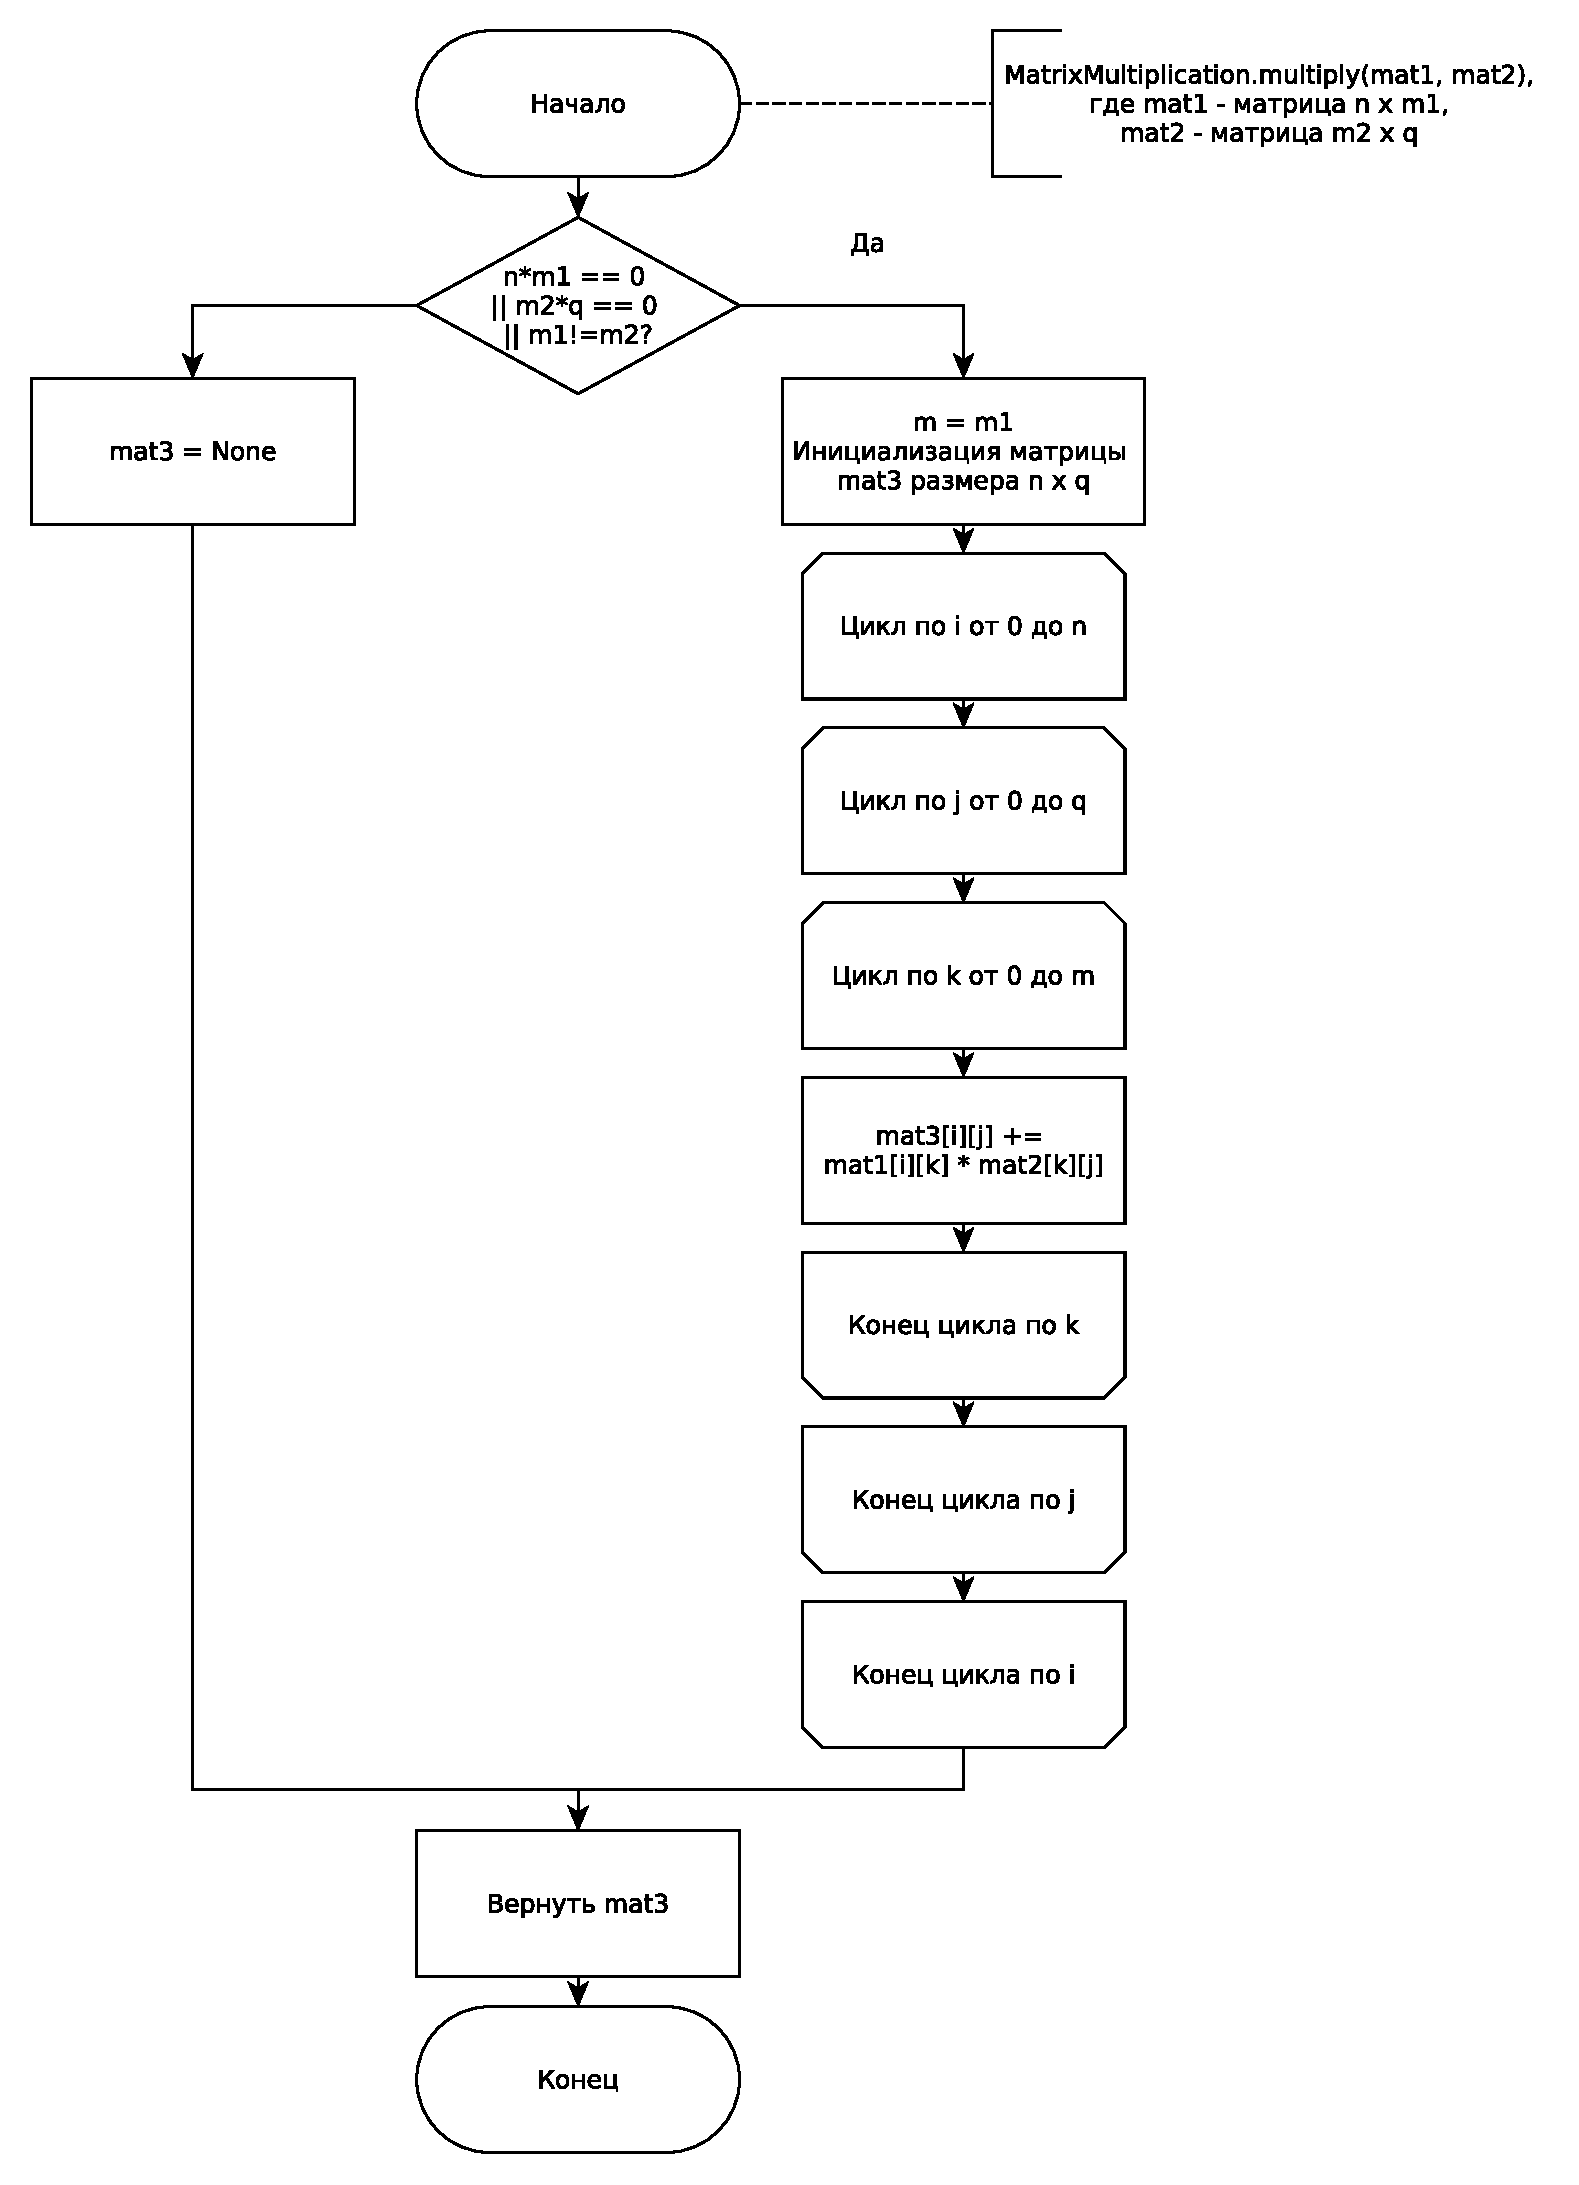
\includegraphics[width=0.85\linewidth]{img/MatrixMultiplication}
        \caption{
            \begin{center}
                Схема стандартного алгоритма умножения матриц
            \end{center}}
        \label{fig:matmult}
    \end{figure}


    \section{Вывод}
    В данном разделе на основе приведенных в аналитическом разделе теоретических данных
    были составлены схемы алгоритмов для реализации в технологической части.
    Были составлены схемы разделения вычисления определителя на потоки.
    \newpage


    \chapter{Технологическая часть}
    Данный раздел содержит обоснование выбора языка и среды разработки, реализацию алгоритмов.


    \section{Требования к программному обеспечению}
    Требования, выдвигаемые к разрабатываемому ПО:
    \begin{itemize}
        \item входные данные - размеры двух матриц, их элементы;
        \item выходные данные - матрица, являющаяся произведением первой входной матрицы на вторую.
    \end{itemize}


    \section{Средства реализации}
    Для реализации программы был выбран язык программирования Python~\cite{Python}.
    Такой выбор обусловлен следующими причинами:
    \begin{itemize}
        \item имеется большой опыт разработки;
        \item удобные средства для работы с потоками;
        \item обладает информативной документацией.
    \end{itemize}


    \section{Реализация алгоритмов}
    В листингах~\ref{code:} -~\ref{code:} представлены
    реализации рассматриваемых алгоритмов.


    \section{Тестирование}
    В таблице \ref{tab:tests} представлены использованные для тестирования методом "черного ящика" данные,
    были рассмотрены все возможные тестовые случаи. Все тесты пройдены успешно.

    \begin{table}[h]
        \begin{center}
            \captionsetup{justification=raggedleft, singlelinecheck=false}
            \caption[]{\label{tab:tests} Проведенные тесты}
            \begin{tabular}{c@{\hspace{7mm}}c@{\hspace{7mm}}c@{\hspace{7mm}}c@{\hspace{7mm}}c@{\hspace{7mm}}c@{\hspace{7mm}}}
                \hline
                Матрица 1 & Строка 1 & Ожидаемый результат\\ [0.5ex]
                \hline
                $\begin{pmatrix}
                     1 & 5 & 2 \\
                     1 & 2 & 8 \\
                     1 & 3 & 2
                \end{pmatrix}$ &
                $\begin{pmatrix}
                     1  & 4  & 9  \\
                     8  & 8  & 8  \\
                     12 & 21 & 13
                \end{pmatrix}$ &
                $\begin{pmatrix}
                     65  & 86  & 75  \\
                     113 & 188 & 129 \\
                     49  & 70  & 59
                \end{pmatrix}$ \\
                \vspace{2mm}
                \vspace{2mm}
                $\begin{pmatrix}
                     9 & 8 & 7 \\
                     6 & 5 & 4
                \end{pmatrix}$ &
                $\begin{pmatrix}
                     3 \\
                     2 \\
                     1
                \end{pmatrix}$ &
                $\begin{pmatrix}
                     50 \\
                     32
                \end{pmatrix}$ \\
                \vspace{2mm}
                \vspace{2mm}
                $\begin{pmatrix}
                     12
                \end{pmatrix}$ &
                $\begin{pmatrix}
                     17
                \end{pmatrix}$ &
                $\begin{pmatrix}
                     204
                \end{pmatrix}$ \\
                \vspace{2mm}
                \vspace{2mm}
                $\begin{pmatrix}
                     -1 & -2 & 3 \\
                     8  & -9 & 7 \\
                     -4 & -7 & 5
                \end{pmatrix}$ &
                $\begin{pmatrix}
                     1 & 2 & 3  \\
                     4 & 5 & 6  \\
                     7 & 8 & -9
                \end{pmatrix}$ &
                $\begin{pmatrix}
                     12 & 12 & -42 \\
                     21 & 27 & -93 \\
                     3  & -3 & -99
                \end{pmatrix}$ \\
                \vspace{2mm}
                \vspace{2mm}
                $\begin{pmatrix}
                     8 & 7
                \end{pmatrix}$ &
                $\begin{pmatrix}
                     4 & 2
                \end{pmatrix}$ &
                Ошибка \\
                \vspace{2mm}
                \vspace{2mm}
                $\begin{pmatrix}
                     1  & -1 & 2  \\
                     -4 & 7  & -5
                \end{pmatrix}$ &
                $\begin{pmatrix}
                     1 & 8  & 3 \\
                     6 & -9 & 7 \\
                     1 & 4  & 8
                \end{pmatrix}$ &
                $\begin{pmatrix}
                     -3 & 25   & 12 \\
                     33 & -115 & -3
                \end{pmatrix}$ \\
                \vspace{2mm}
                \vspace{2mm}
                $\begin{pmatrix}
                     0 & 0 & 0 \\
                     0 & 0 & 0 \\
                     0 & 0 & 0
                \end{pmatrix}$ &
                $\begin{pmatrix}
                     1 & 8 & 6  \\
                     3 & 5 & -4 \\
                     6 & 6 & 6
                \end{pmatrix}$ &
                $\begin{pmatrix}
                     0 & 0 & 0 \\
                     0 & 0 & 0 \\
                     0 & 0 & 0
                \end{pmatrix}$ \\
                \vspace{2mm}
                \vspace{2mm}
                $\begin{pmatrix}
                     1 & 4  \\
                     8 & -3
                \end{pmatrix}$ &
                $\begin{pmatrix}
                     0 & 0 \\
                     0 & 0
                \end{pmatrix}$ &
                $\begin{pmatrix}
                     0 & 0 \\
                     0 & 0
                \end{pmatrix}$ \\
                \vspace{2mm}
                \vspace{2mm}
                $\begin{pmatrix}
                     1 & 0 & 0 & 0 \\
                     0 & 1 & 0 & 0 \\
                     0 & 0 & 1 & 0 \\
                     0 & 0 & 0 & 1
                \end{pmatrix}$ &
                $\begin{pmatrix}
                     4  & 8 & -9 & 5 \\
                     -8 & 7 & 9  & 0 \\
                     7  & 9 & -1 & 1 \\
                     8  & 5 & 2  & 8
                \end{pmatrix}$ &
                $\begin{pmatrix}
                     4  & 8 & -9 & 5 \\
                     -8 & 7 & 9  & 0 \\
                     7  & 9 & -1 & 1 \\
                     8  & 5 & 2  & 8
                \end{pmatrix}$ \\
                \vspace{2mm}
                \vspace{2mm}
                $\begin{pmatrix}
                     7  & 1  & 3  \\
                     -1 & -1 & -1 \\
                     3  & 5  & 2
                \end{pmatrix}$ &
                $\begin{pmatrix}
                     1 & 0 & 0 \\
                     0 & 1 & 0 \\
                     0 & 0 & 1
                \end{pmatrix}$ &
                $\begin{pmatrix}
                     7  & 1  & 3  \\
                     -1 & -1 & -1 \\
                     3  & 5  & 2
                \end{pmatrix}$
                \vspace{2mm}
                \vspace{2mm}

            \end{tabular}
        \end{center}
    \end{table}\\


    \section{Вывод}
    В данном разделе были реализованы и протестированы алгоритмы умножения матриц: классический, Копперсмита-Винограда и оптимизированный Копперсмита-Винограда.
    \newpage


    \chapter{Экспериментальная часть}
    В данном разделе сравниваются реализованные алгоритмы, дается сравнительная оценка затрат на память и время.


    \section{Пример работы программы}
    Пример работы программы представлен на рисунках~\ref{fig:work_example1}-\ref{fig:work_example1}.
    \captionsetup{singlelinecheck=true}
    \begin{figure}[H]
        \centering
        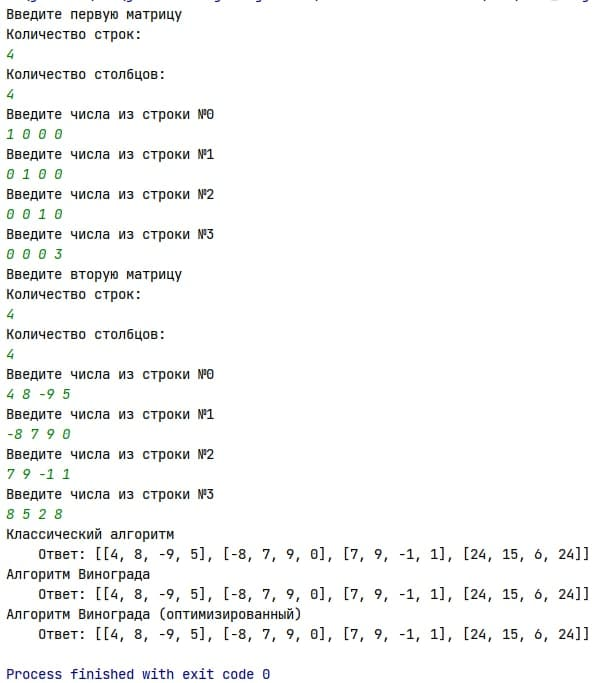
\includegraphics[width=0.7\linewidth]{images/example1}
        \caption{Ввод данных}
        \label{fig:work_example1}
    \end{figure}

    \begin{figure}[H]
        \centering
        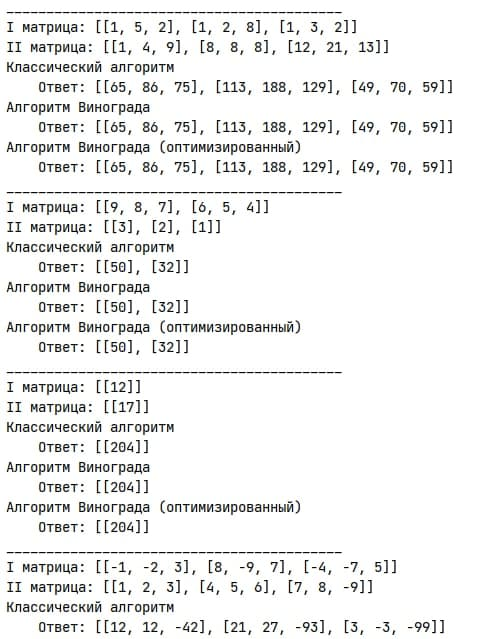
\includegraphics[width=0.7\linewidth]{images/example2}
        \caption{Результат работы программы}
        \label{fig:work_example2}
    \end{figure}


    \section{Технические характеристики}
    Технические характеристики устройства, на котором выполнялось тестирование:
    \begin{itemize}
        \item операционная система --- Windows~\cite{windows} 10 64-bit;
        \item оперативная память --- 16 Гб;
        \item процессор --- Intel(R) Core(TM) i5-7600 CPU @ 3.50GHz~\cite{i5}.
    \end{itemize}


    \section{Время выполнения алгоритмов}

    Время выполнения алгоритмов замерялось на автоматически генерируемых
    квадратных матрицах необходимого размера с использованием функции getrusage библиотеки resources.
    Усредненные результаты замеров процессорного времени приведены в таблице.
    Используемые обозначения:
    "Классич."\ - классический алгоритм умножения матриц,
    "Виноград"\ - алгоритм Копперсмита-Винограда,
    "Опт.Виноград"\ - оптимизированный алгоритм Копперсмита-Винограда.

    \begin{table}[h]
        \begin{center}
            \captionsetup{justification=raggedleft, singlelinecheck=false}
            \caption{\label{time} Время обработки строк разной длины в микросекундах}
            \begin{tabular}{|c c c c|}
                \hline
                Размер & Классич. & Виноград & Опт.Виноград\\ [0.5ex]
                \hline
                10     & 7626     & 8432     & 6334         \\
                \hline
                11     & 10114    & 11119    & 8247         \\
                \hline
                30     & 198387   & 200491   & 144975       \\
                \hline
                31     & 221763   & 221463   & 159228       \\
                \hline
                50     & 914673   & 913305   & 651054       \\
                \hline
                51     & 990919   & 975478   & 695120       \\
                \hline
                70     & 2568877  & 2492211  & 1768562      \\
                \hline
                71     & 2692695  & 2625663  & 1855013      \\
                \hline
                90     & 5472335  & 5286995  & 3717559      \\
                \hline
                91     & 5634068  & 5480780  & 3892148      \\
                \hline
                110    & 10070443 & 9613919  & 6775491      \\
                \hline
                111    & 10310690 & 9927475  & 7034633      \\
                \hline
            \end{tabular}
        \end{center}
    \end{table}

    \begin{figure}[H]
        \centering
        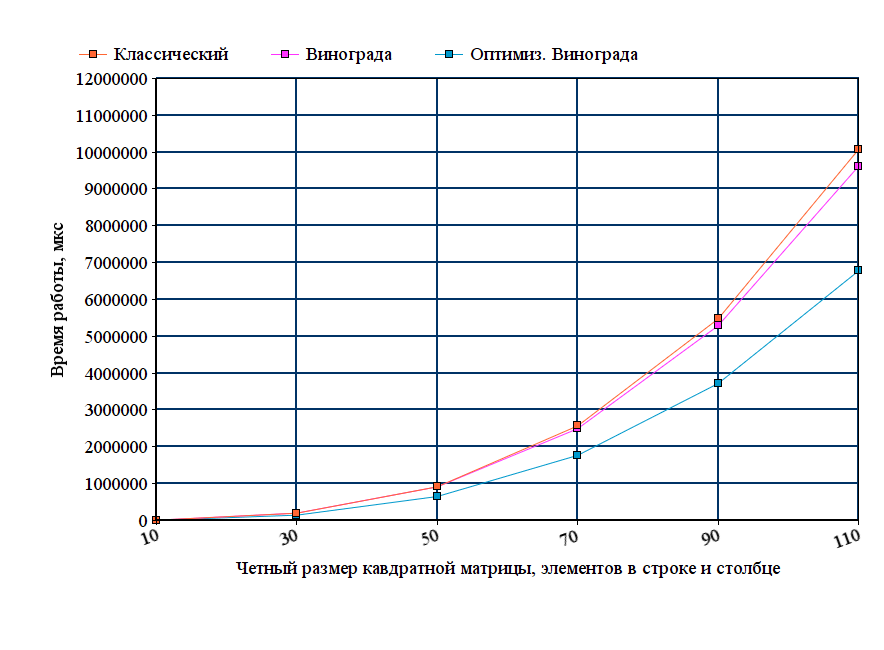
\includegraphics[width=1\linewidth]{images/odd_mat}
        \caption{Сравнение времени работы алгоритмов умножения квадратных матриц четных размеров}
        \label{fig:odd_graph}
    \end{figure}

    \begin{figure}[H]
        \centering
        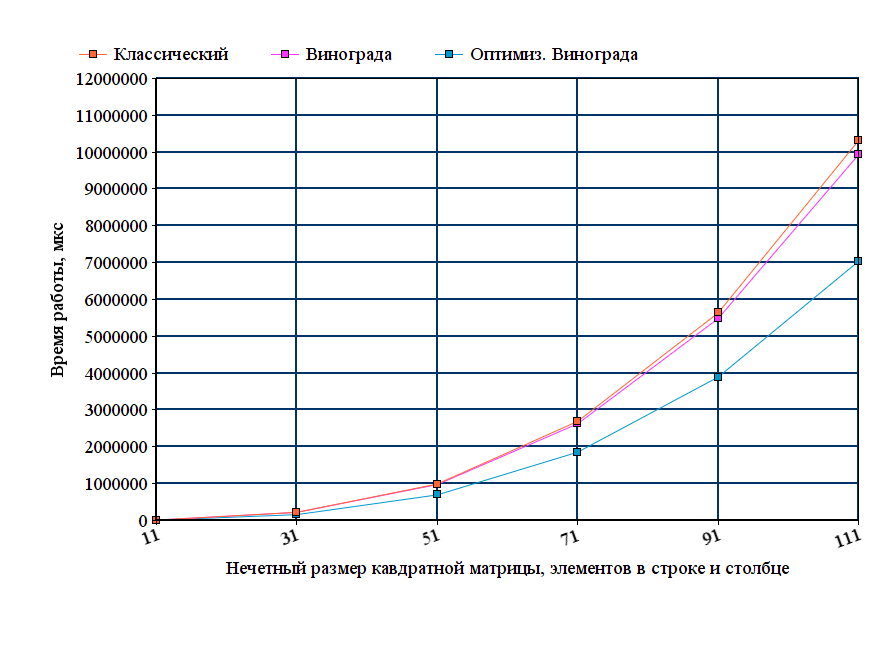
\includegraphics[width=1\linewidth]{images/even_mat}
        \caption{Сравнение времени работы алгоритмов умножения квадратных матриц нечетных размеров}
        \label{fig:even_graph}
    \end{figure}


    \section{Вывод}

    По результатам проведенных замеров видно,
    что оптимизированный алгоритм Копперсмита-Винограда работает в 1.2-1.5 раза быстрее
    классического алгоритма умножения матриц с увеличением этого коэффициента при увеличении размера матрицы.
    Важно заметить, что коэффициент незначительно меньше для матриц нечетных размеров,
    что говорит о более медленной работе оптимизированного алгоритма Винограда для таких матриц,
    в то время как классический алгоритм зависимости от четности размеров не имеет.
    Алгоритм Копперсмита-Винограда на четных матрицах меньше 50x50 работает медленнее классического алгоритма,
    на больших - чуть быстрее, однако разрыв составляет не более 1.05 раз.
    В случае с нечетным размером матрицы алгоритм Винограда на небольших матрицах проигрывает
    классическому алгоритму, но при увеличении размерности время работы обоих алгоритмов сопоставимо,
    с небольшим преимуществом алгоритма Винограда.
    \newpage

    \addcontentsline{toc}{chapter}{Заключение}
    \chapter*{Заключение}
    В процессе выполнения лабораторной работы были изучены и реализованы классический
    алгоритм умножения и алгоритм Копперсмита-Винограда матриц, оптимизирован алгоритм Винограда.

    Согласно проведенному анализу трудоемкости алгоритмов в соответствии
    с выбранной моделью вычислений, трудоемкость классического алгоритма составила
    приблизительно $11mnq$, алгоритма Копперсмита-Винограда - $16mnq$,
    оптимизированного алгоритма Копперсмита-Винограда - $9mnq$.

    Было исследовано процессорное время выполнения выше обозначенных алгоритмов.
    В результате было выявлено, что на матрицах с количеством элементов в строках и столбцах,
    меньших 50, дольше всего работает алгоритм Копперсмита-Винограда, на больших - классический,
    причем время работы алгоритма Винограда незначительно меньше (разница не превышает 1.04 раз).
    Быстрее всего работает оптимизированный алгоритм Копперсмита-Винограда
    (в 1.2-1.5 раз быстрее других алгоритмов с увеличением разницы во времени работы с увеличением размеров матриц),
    однако заметна небольшая деградация времени работы для матриц с нечетным
    количеством строк и столбцов (как и у алгоритма Винограда-Копперсмита),
    тогда как классический алгоритм таким свойством не обладает.


    \newpage
    \addcontentsline{toc}{chapter}{Литература}

    \bibliographystyle{utf8gost705u}  % стилевой файл для оформления по ГОСТу
    \bibliography{report_4}          % имя библиографической базы (bib-файла)

\end{document}